\printMiniToc


\section{Objectifs du TM}
\label{sec:objectifsTM}
Durant ce Travail de Maturité, je tenterai de réaliser un  jeu vidéo -- ou plutôt une version de démonstration (abrégée \enquote{demo}\definition) -- en 3 dimensions, nommé \nomJeu. Mon objectif sera de comprendre ce qui fait un bon jeu vidéo: graphisme, story-telling\definition, scénario, musique. Il me faudra trouver les outils nécessaires (éditeur d'image, éditeur 3D, moteur de jeu, langages de programmation) et passer à la réalisation pratique.

Mais plus que réaliser un jeu vidéo parmi déjà tant d'autres, je m'efforcerai de conférer un sens à l'histoire, d'ajouter des critiques et des pensées sur notre monde. En effet, pourquoi le livre serait-il le moyen d'expression le plus utilisé quand un jeu vidéo peut faire de même, l'interactivité -- pour ne pas dire le fun -- en plus? Certains titres déjà sortis comme \textit{Mortal Combat} ou le plus moderne \textit{Call of Duty} ont certainement contribué à la création d'une réputation négative qui aura empêché que des jeux plus philosophiques ou critiques n'apparaissent. L'ajout d'une nouvelle dimension plus intellectuelle à ce média sera donc un objectif principal de ce travail.



\section{Motivations personnelles}
Le monde des jeux vidéo m'a toujours passionné. Il est, pour moi, une brèche dans la vie de tous les jours, un moyen de s'échapper de notre quotidien, de vivre des histoires extraordinaires dans des univers fantastiques. La diversité des jeux est telle, que chacun peut y trouver son bonheur; ils font travailler notre imagination, testent nos réflexes, nous détendent et nous font réfléchir. Et s'ils sont des divertissements très efficaces, ils sont aussi, bien que cela ait été relégué au deuxième plan jusqu'ici, des moyens d'expression redoutables.

Par ailleurs, depuis ma première année au collège, je me suis intéressé à l'informatique. J'ai ainsi touché à la robotique, la programmation, la modélisation 3D, la retouche photo, aux réseaux et à d'autres domaines techniques.

Ces deux éléments m'ont donné l'envie et la possibilité de me lancer dans la réalisation d'un jeu vidéo. Je me suis documenté sur ce genre de projet: quels outils utiliser? quel langage de programmation employer? en 2 ou 3 dimensions? Mais l'ampleur et la complexité d'une telle création m'ont rapidement arrêté et j'ai abandonné l'idée pour me concentrer sur d'autres programmes plus réalisables... jusqu'au moment de définir le sujet de mon TM. Il me fallait un projet suffisamment vaste et complexe pour m'intéresser durant une année. Quel meilleur choix que la réalisation d'un jeu vidéo!



\section{Les jeux vidéo}
\index{Jeux vidéo}
\subsection{Définition}
Même si tout le monde a au moins une petite idée de ce qu'est un jeu vidéo, il me paraît important de rappeler la définition que Wikipédia donne à ce sujet et de la compléter. Selon l'encyclopédie en ligne:

\begin{displayquote}
\enquote{Un jeu vidéo est un jeu électronique qui implique une interaction humaine avec une interface utilisateur dans le but de générer un retour visuel sur un dispositif vidéo. Le joueur de jeu vidéo dispose de périphériques pour agir sur le jeu et percevoir les conséquences de ses actes sur l'environnement virtuel. Le mot « vidéo » dans le jeu vidéo, fait traditionnellement référence à un dispositif d'affichage de trame, mais à la suite de la vulgarisation du terme, il implique désormais tout type de dispositif d'affichage.}\cite{Jeuvideo_}
\end{displayquote}

Cette définition, très complète du point de vue technique, fait cependant abstraction de la partie humaine des jeux vidéo. Ils sont bien, d'un point de vue purement logique, des interactions homme-machine. Mais ils sont aussi, et pour moi avant tout, une façon de se divertir, de découvrir, d'imaginer et même de partager (jeux multijoueurs). Pour qu'un jeu ait du succès, il doit faire ressentir aux joueurs des émotions, il doit communiquer une histoire, stimuler notre réactivité, nos capacités de réflexion et de logique. Un jeu vidéo, c'est aussi l'occasion de rêver, de vivre des aventures dans d'autres mondes, tout comme un livre, à cette différence près que la narration y est interactive.

Au cours de ce travail, j'aborderai ces différents aspects: la partie humaine sera approfondie dans les premiers chapitres avec la création du monde, le scénario et le gameplay\definition; la partie technique le sera dans les derniers chapitres avec la création des niveaux, la réalisation pratique et, finalement, la diffusion du jeu.


%\subsection{Les jeux vidéo au fil des années}
%
%\begin{minipage}[t]{.48\textwidth}
%	\subsubsection{1970}
%	\begin{figure}[H]
%		\captionsetup{format=myformat}
%		\center
%		\vspace*{-1\baselineskip}
%		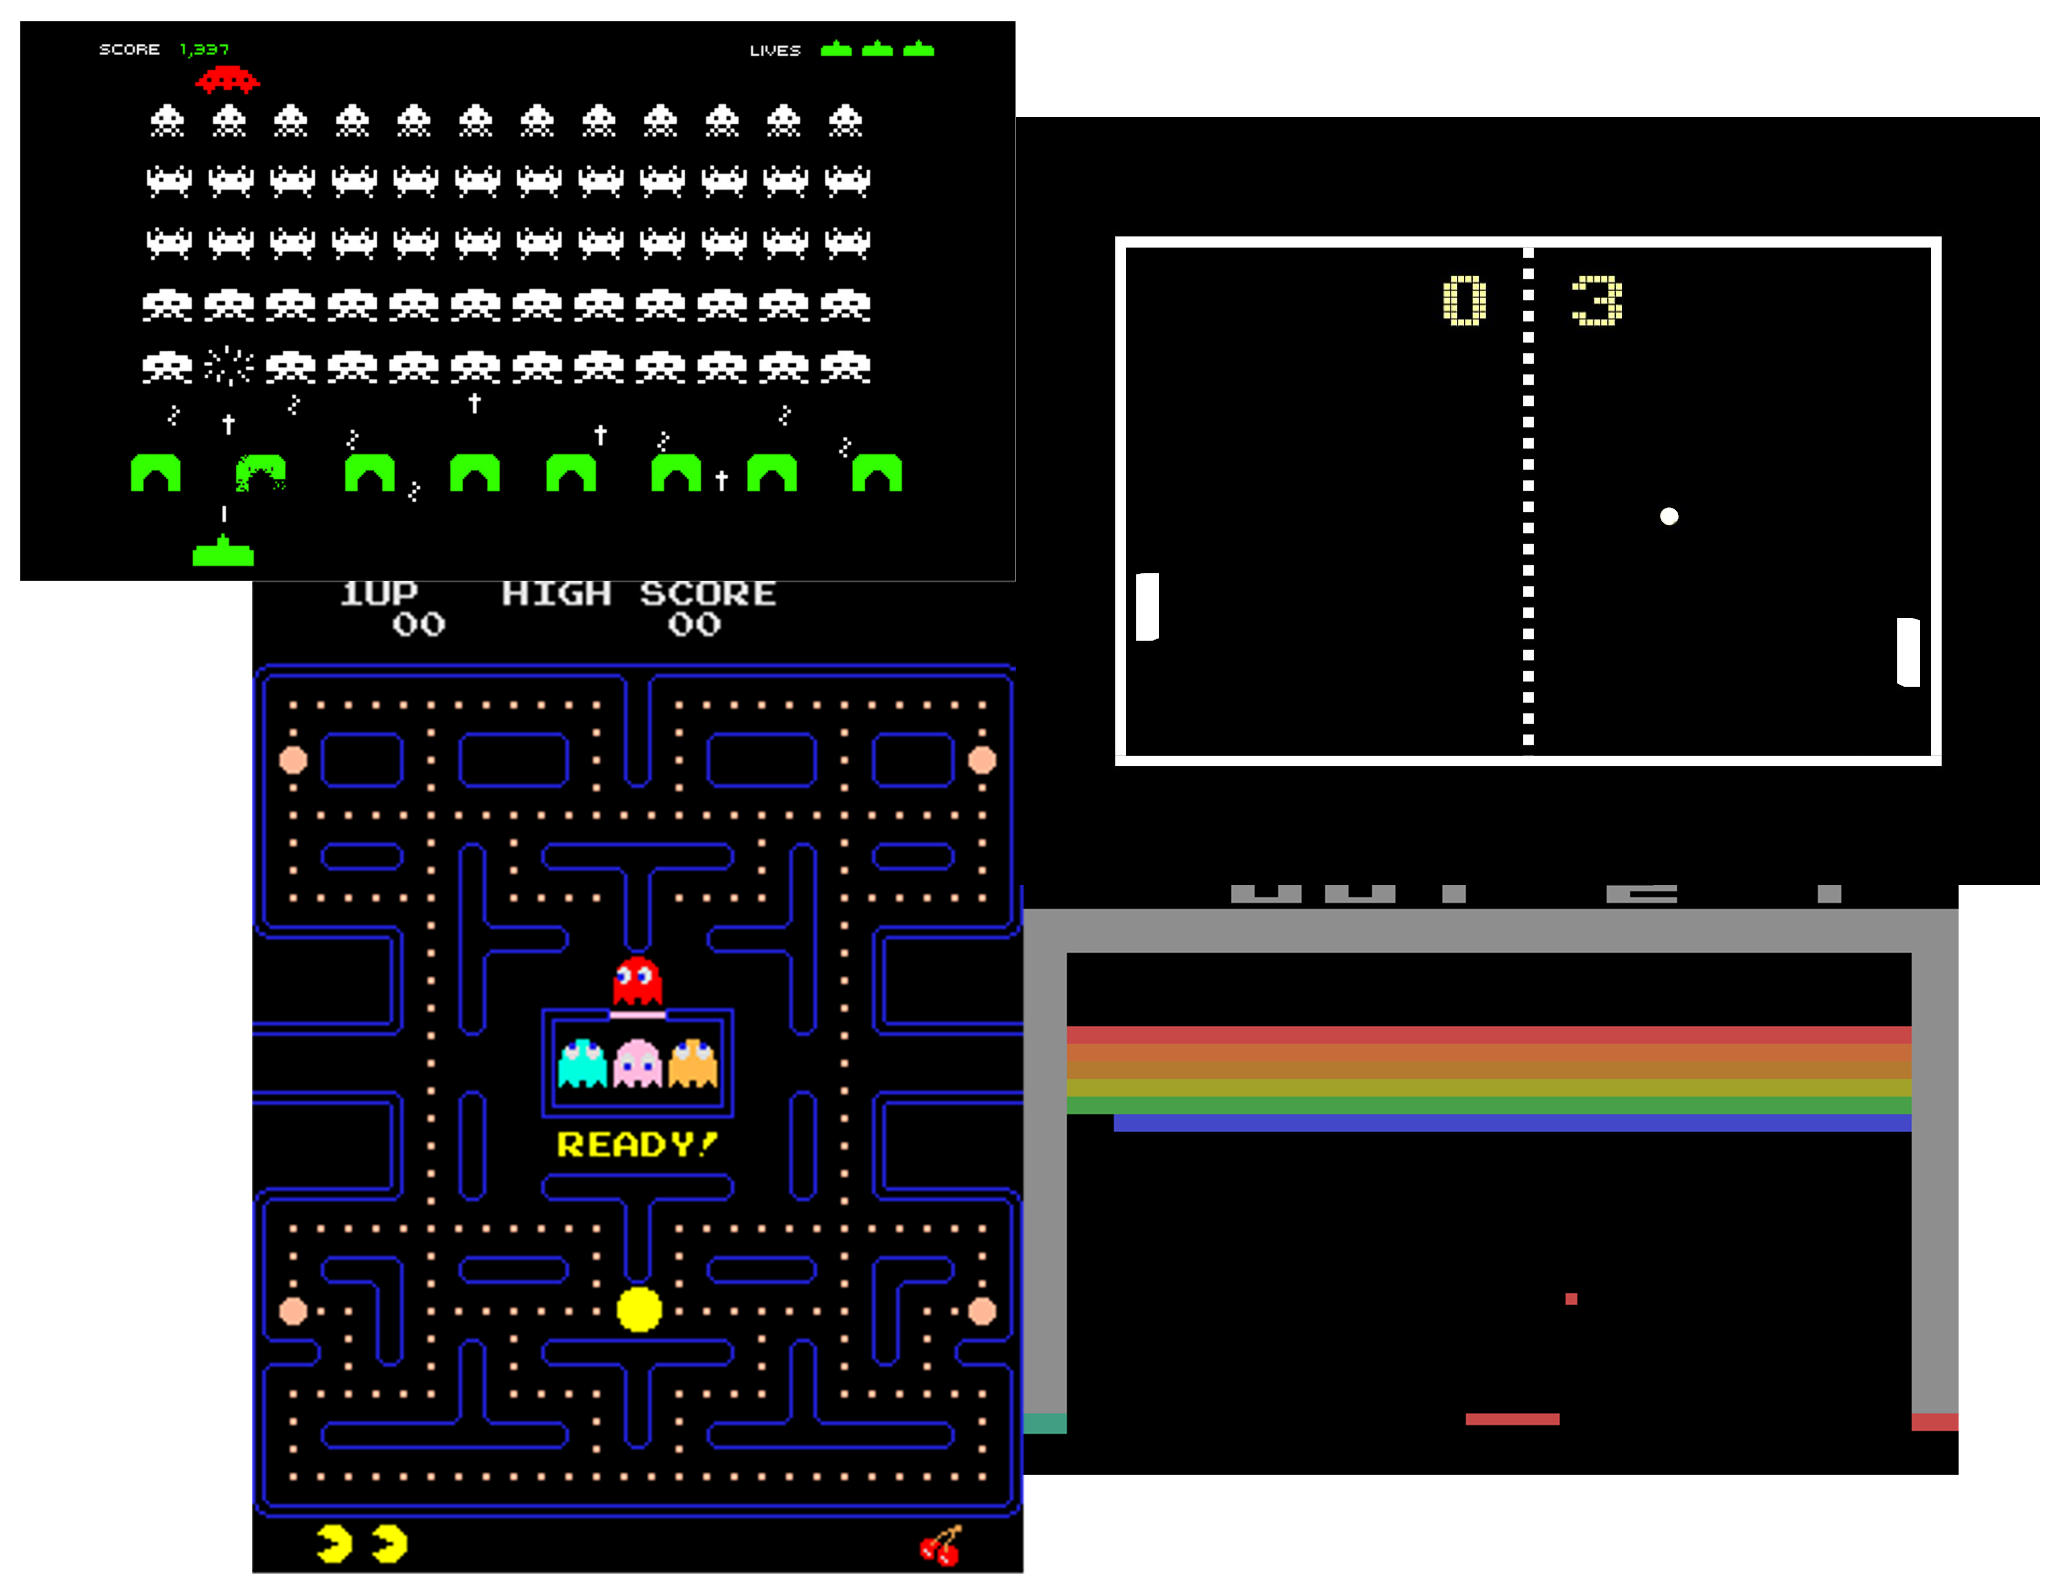
\includegraphics[width=\linewidth]{./images/Introduction/imagdle1970.png}
%		\caption{Space Invaders, Pong,\\ Pacman et Breakout}
%	\end{figure}	
%\end{minipage}\hspace{.04\textwidth}\begin{minipage}[t]{.48\textwidth}
%	\subsubsection{1980}
%	\vspace*{-1\baselineskip}
%	\begin{figure}[H]
%		\center
%		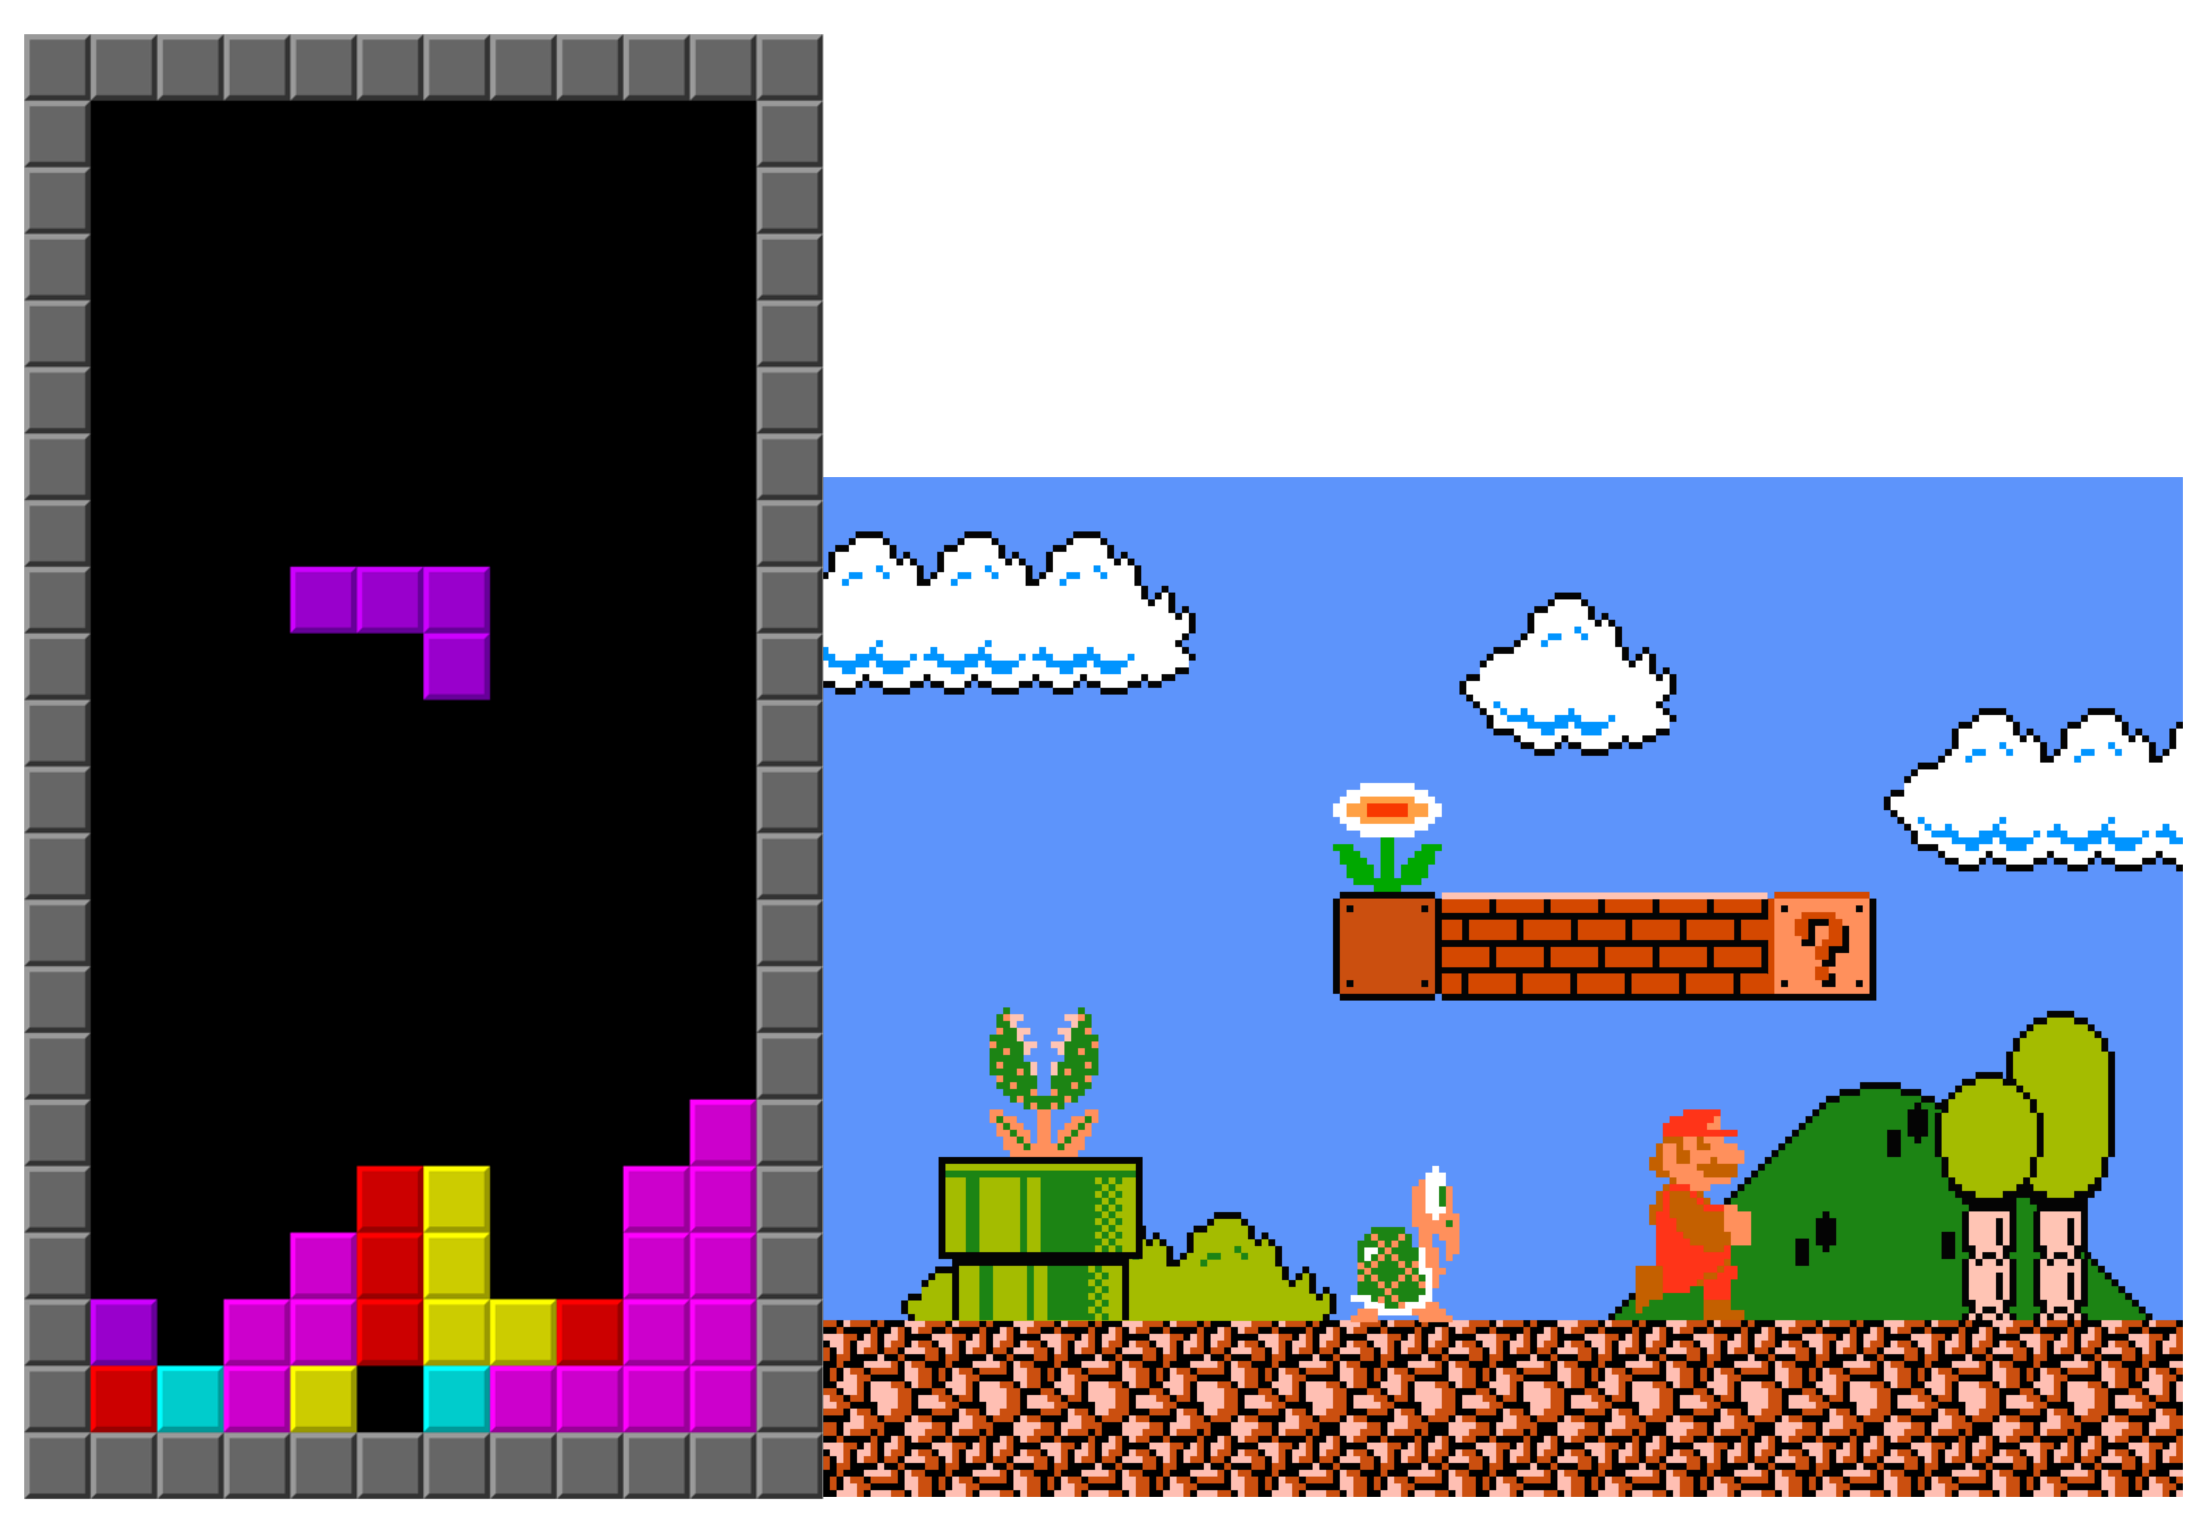
\includegraphics[width=\linewidth]{./images/Introduction/imagdle1980.png}
%		\caption{Tetris et Super Mario Bros}
%	\end{figure}
%\end{minipage}
%
%\begin{minipage}[t]{.48\textwidth}
%	\subsubsection{1990}
%	\vspace*{-1\baselineskip}
%	\begin{figure}[H]
%		\captionsetup{format=myformat}
%		\center
%		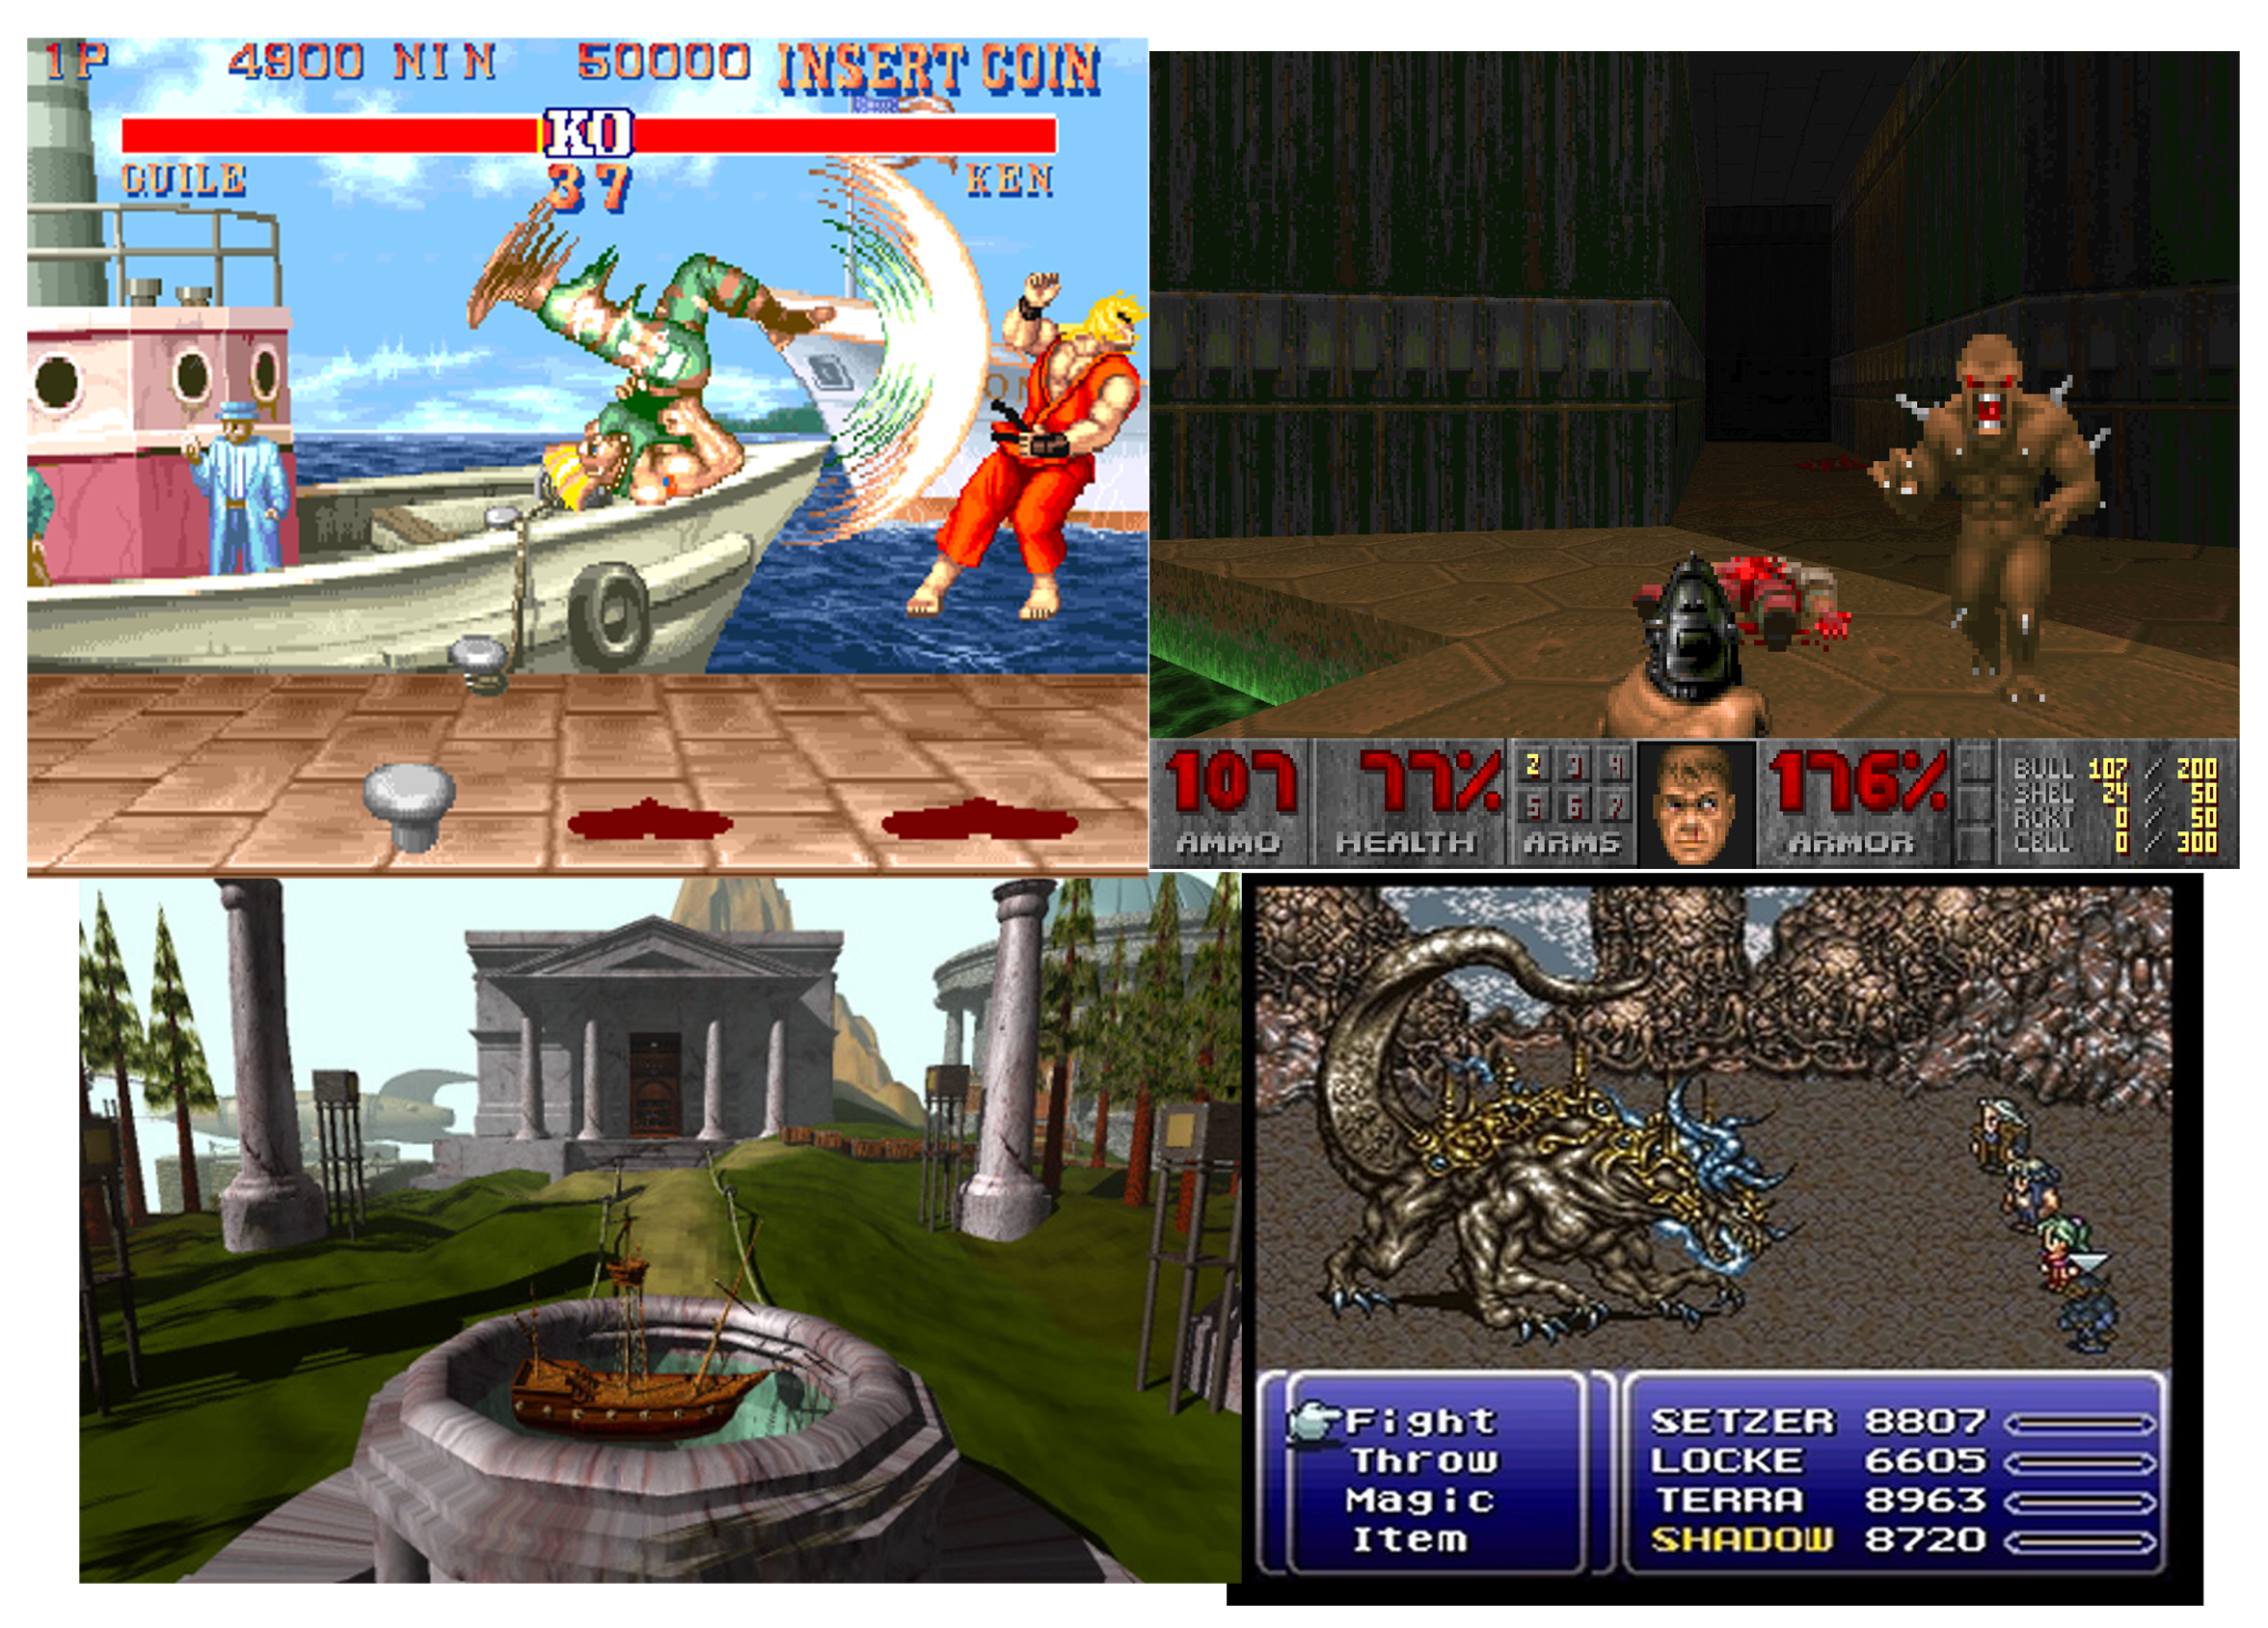
\includegraphics[width=\linewidth]{./images/Introduction/imagdle1990.png}
%		\caption{Street Fighter II, Doom,\\ Myst et Final Fantasy VI}
%	\end{figure}
%\end{minipage}\hspace{.04\textwidth}\begin{minipage}[t]{.48\textwidth}
%	\subsubsection{2000 à maintenant}
%	\vspace*{-1\baselineskip}
%	\begin{figure}[H]
%		\captionsetup{format=myformat}
%		\center
%		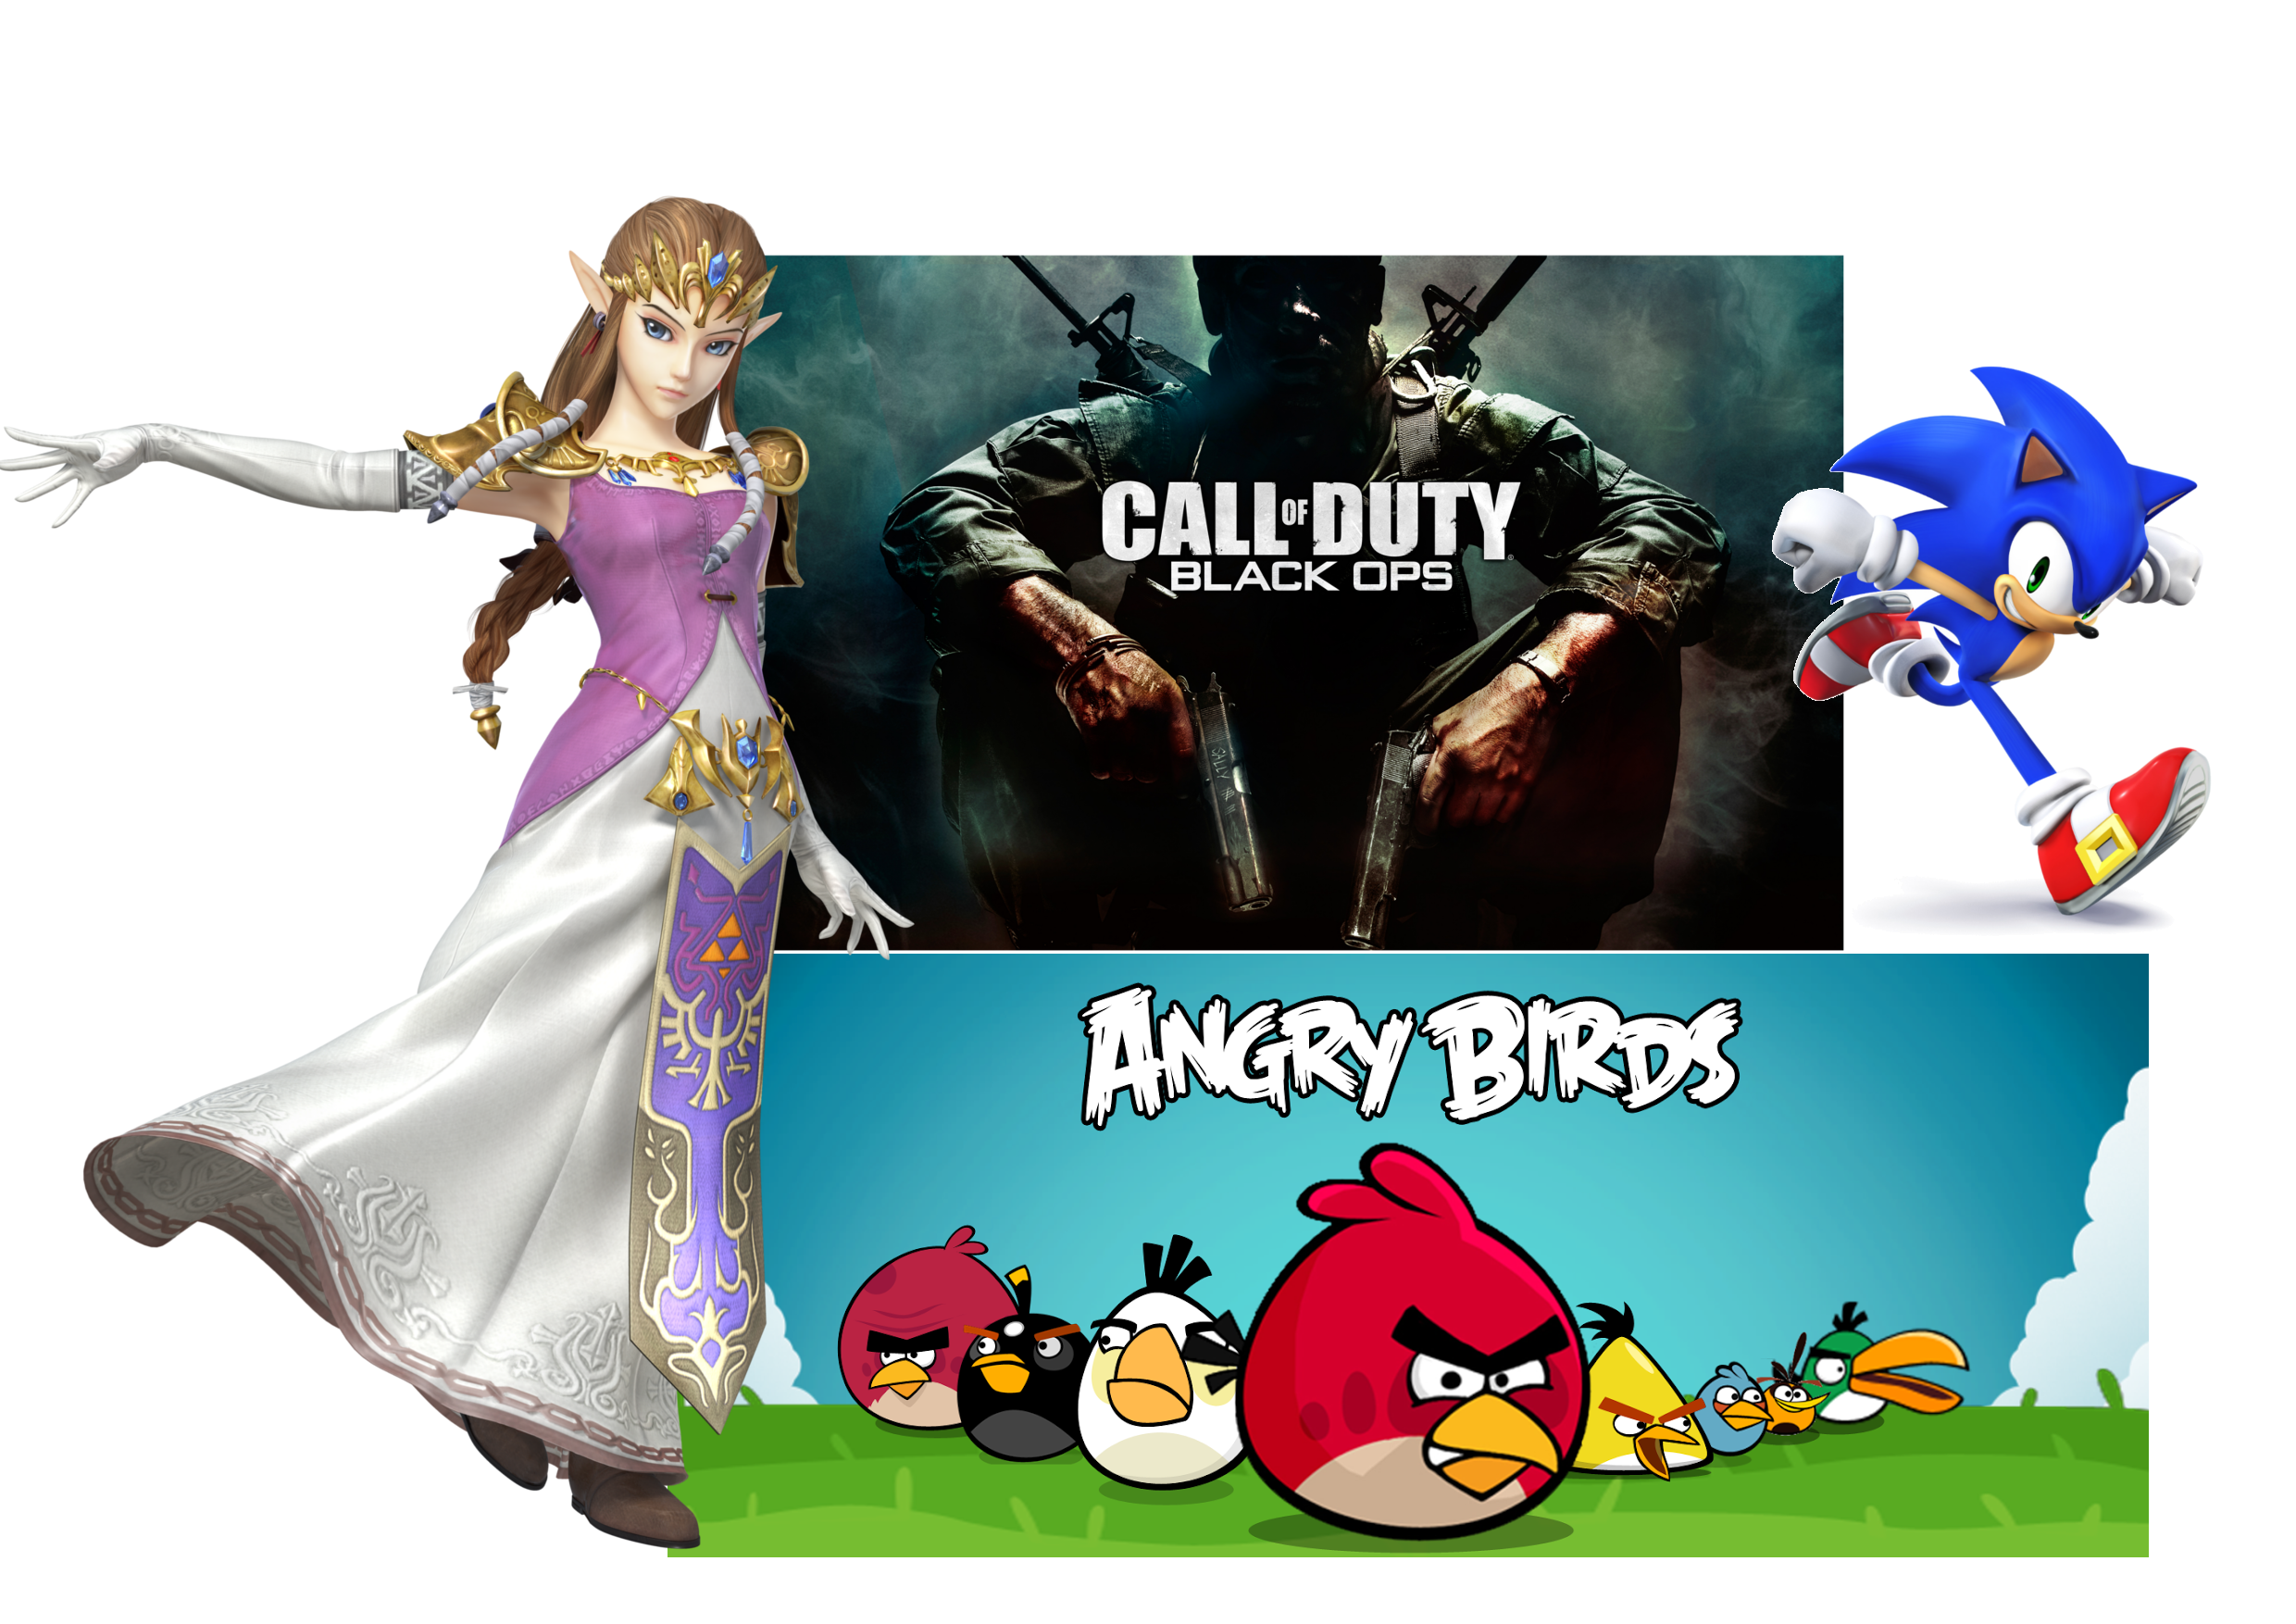
\includegraphics[width=\linewidth]{./images/Introduction/imagdle2000.png}
%		\caption{Zelda, Call of Duty,\\Sonic et Angry Birds}
%	\end{figure}
%\end{minipage}
%\vspace{\baselineskip}


\section{Utilisation de logiciels}

La réalisation d'un tel travail nécessite forcément un nombre important de logiciels. Mais tous les logiciels sont-ils bons à utiliser ou plus simplement, sont-ils tous utilisables? Définissons tout d'abord les deux types principaux de logiciels.

\subsection{Les logiciels, libres ou propriétaires?}
Un logiciel libre désigne un programme dont le code source est accessible. Cela permet à la communauté entourant ce programme d'apporter des améliorations et de le partager légalement avec le reste du monde. Ces programmes tendent à être gratuits mais ne le sont pas forcément. On parle aussi de logiciels \enquote{open source}; ce terme désigne également des logiciels libres, mais si la désignation \enquote{libre} s'intéresse à l'aspect philosophique et politique, \enquote{open source} se rapporte à la partie technique ainsi qu'à la diffusion du programme. Parmi les logiciels libres, on pourra trouver par exemple: Linux, Firefox, Thunderbird, Gimp, Blender et Libre Office.\cite{Logiciellibre_}\cite{Opensource_}

L'opposé du logiciel libre est le logiciel propriétaire. Ces programmes sont très largement majoritaires dans l'univers informatique d'aujourd'hui et se définissent par leur code source inaccessible au public. Citons par exemple: Microsoft Windows, la suite Microsoft Office, tous les logiciels Apple et la suite Adobe à laquelle appartient Photoshop. Certains d'entre eux peuvent être gratuits mais c'est l'inverse qui se vérifie le plus souvent.

\subsection{Quels logiciels utiliser?}
La réalisation d'un jeu vidéo se fait normalement sur plusieurs années, avec une équipe de professionnels et des budgets importants -- pour ne pas dire colossaux, suivant les titres. Mes ressources sont évidemment plus limitées: je suis seul, dispose de moins d'une année et surtout, mon budget est nettement plus restreint.

De plus, le logiciel libre est, pour moi, une des révolutions les plus importantes et bénéfiques de l'ère moderne de l'informatique. C'est un modèle économique complètement différent, basé sur l'entraide et, le plus souvent, la gratuité. C'est une autre façon, un peu à la manière d'Internet, de rendre la connaissance gratuite et disponible pour tous.

Pour toutes ces raisons, je m'efforcerai de n'employer que des logiciels gratuits et tenterai le plus possible d'utiliser des programmes libres pour soutenir ce mouvement.
